\section{Experimental Validation}
\label{S:Exp}



\begin{figure}[H]
\centering
\subfigure[The test geometry, robot paths, and encounters (gray).]{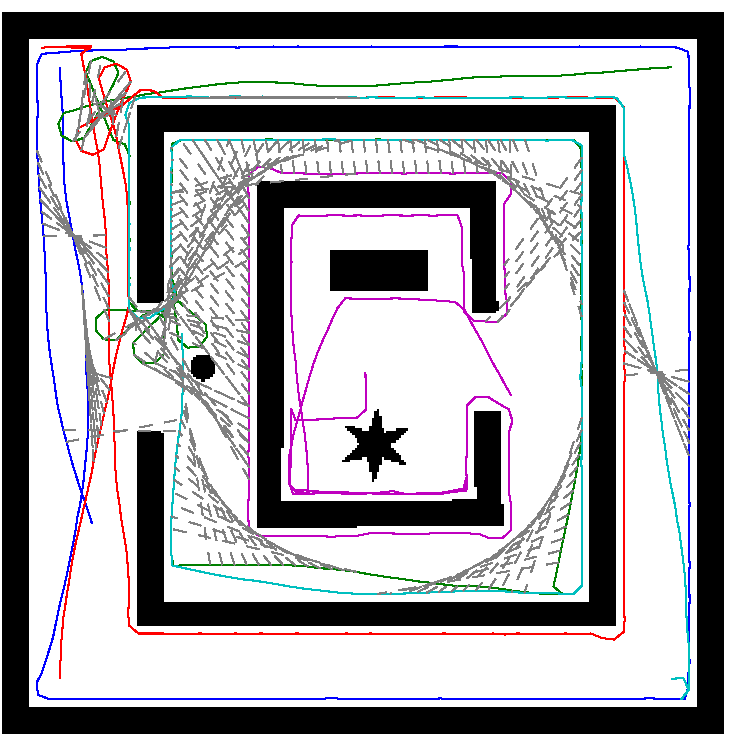
\includegraphics{../FinalFigures/Encounters}}
\subfigure[Robot encounters at a given time.]{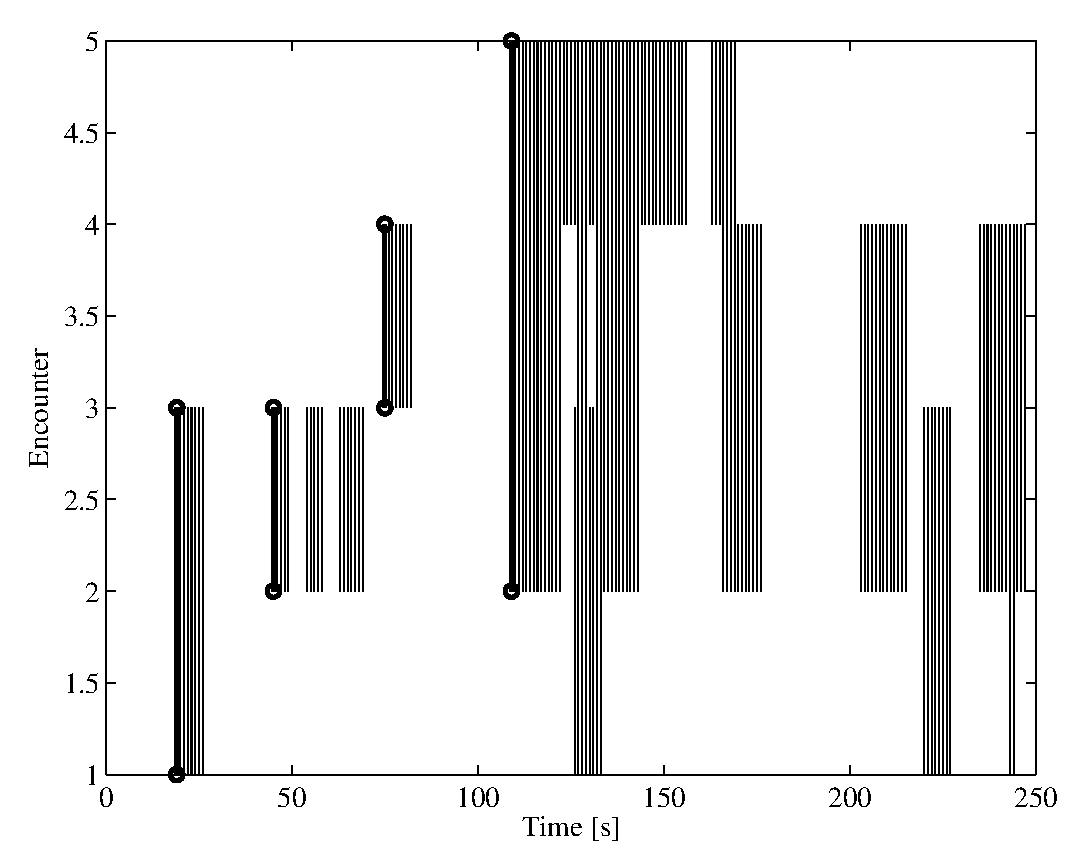
\includegraphics{../FinalFigures/EncountersTimes}}
\end{figure}



\begin{equation}
\begin{bmatrix}
x_{t}\\
y_{t}
\theta_{t}
\end{bmatrix}=\begin{bmatrix}
x_{t-1}\\
y_{t-1}
\theta_{t-1}
\end{bmatrix}+\begin{bmatrix}
dx_t \cos(\theta_t+d\theta_t)
dy_{t}\sin(\theta_t+d\theta_t)
\theta_{t-1}+d\theta_t
\end{bmatrix}
\end{equation}

%\begin{figure*}[h]
%\centering
%\subfigure[Howard Implementation: Known Poses.]{\includegraphics[width=3in]{../FiguresAndMovies/Howard-NoNoise}}
%\subfigure[Proposed Implementation: Known Poses]{\includegraphics[width=3in]{../FiguresAndMovies/Our-NoNoise}}\\
%\subfigure[Howard Implementation: Unknown Poses, low noise.]{\includegraphics[width=3in]{../FiguresAndMovies/Howard-LowNoise}}
%\subfigure[Proposed Implementation: Unknown Poses, low noise.]{\includegraphics[width=3in]{../FiguresAndMovies/Our-LowNoise}}\\
%\subfigure[Howard Implementation: Unknown Poses, High noise.]{\includegraphics[width=3in]{../FiguresAndMovies/Howard-HighNoise}}
%\subfigure[Proposed Implementation: Unknown Poses, High noise.]{\includegraphics[width=3in]{../FiguresAndMovies/Our-NoNoise}}
%\caption{Comparison between Howard's implementation and the proposed implementation.}
%\end{figure*}


